\documentclass[tikz,border=3pt]{standalone}
\usepackage{fontspec}
\setmainfont{TeX Gyre Termes}
\usepackage{amsmath}
\usepackage{tikz}
\usetikzlibrary{arrows.meta,positioning,fit,backgrounds,calc}

\begin{document}
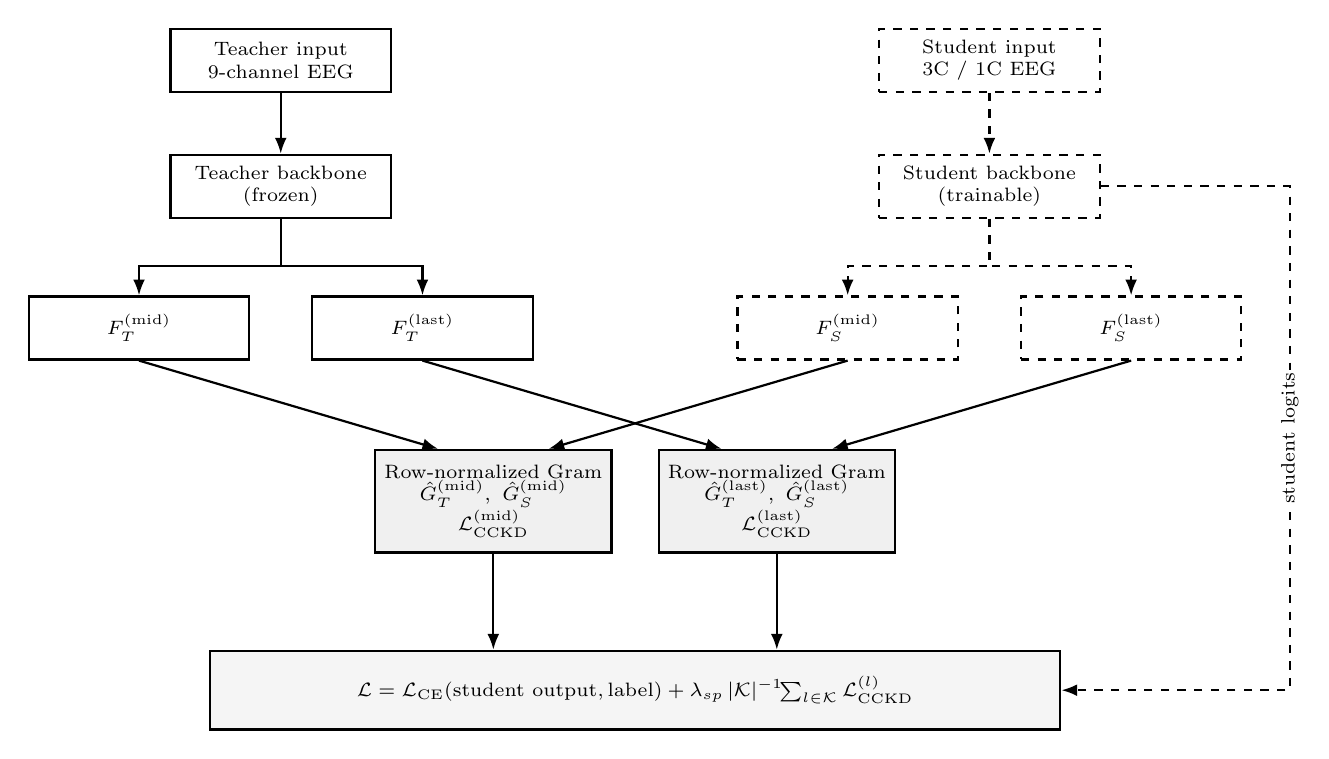
\begin{tikzpicture}[
    x=1mm, y=1mm,
    every node/.style={font=\scriptsize, text=black},
    block/.style={draw=black, thick, rectangle, sharp corners, minimum height=8mm, minimum width=28mm,
                  align=center, fill=white, inner sep=2pt},
    tblock/.style={block},
    sblock/.style={block, dashed},
    lossblock/.style={block, fill=black!6, minimum width=30mm, minimum height=13mm},
    arr/.style={-{Latex[length=2mm]}, thick, draw=black},
    tarr/.style={arr},
    sarr/.style={arr, dashed},
    lossarr/.style={arr},
]

% --- Teacher branch (left column, x = 0) ---
\node[tblock]                       (teacher-in)   at (0, 60)  {Teacher input\\9-channel EEG};
\node[tblock]                       (teacher-net)  at (0, 44)  {Teacher backbone\\(frozen)};
\node[tblock]                       (teacher-mid)  at (-18, 26) {$F_T^{(\mathrm{mid})}$};
\node[tblock]                       (teacher-last) at (18, 26)  {$F_T^{(\mathrm{last})}$};

% --- Student branch (right column, x = 90) ---
\node[sblock]                       (student-in)   at (90, 60) {Student input\\3C / 1C EEG};
\node[sblock]                       (student-net)  at (90, 44) {Student backbone\\(trainable)};
\node[sblock]                       (student-mid)  at (72, 26)  {$F_S^{(\mathrm{mid})}$};
\node[sblock]                       (student-last) at (108, 26) {$F_S^{(\mathrm{last})}$};

\draw[tarr] (teacher-in) -- (teacher-net);
\draw[tarr] (teacher-net.south) -- ++(0,-6) -| (teacher-mid.north);
\draw[tarr] (teacher-net.south) -- ++(0,-6) -| (teacher-last.north);
\draw[sarr] (student-in) -- (student-net);
\draw[sarr] (student-net.south) -- ++(0,-6) -| (student-mid.north);
\draw[sarr] (student-net.south) -- ++(0,-6) -| (student-last.north);

% --- Gram + relational loss, one box per level, each centered between its two taps ---
\node[lossblock] (gram-mid)
  at ($(teacher-mid)!0.5!(student-mid) + (0,-22)$)
  {Row-normalized Gram\\$\hat{G}_T^{(\mathrm{mid})},\ \hat{G}_S^{(\mathrm{mid})}$\\$\mathcal{L}_{\text{CCKD}}^{(\mathrm{mid})}$};
\node[lossblock] (gram-last)
  at ($(teacher-last)!0.5!(student-last) + (0,-22)$)
  {Row-normalized Gram\\$\hat{G}_T^{(\mathrm{last})},\ \hat{G}_S^{(\mathrm{last})}$\\$\mathcal{L}_{\text{CCKD}}^{(\mathrm{last})}$};

\draw[lossarr] (teacher-mid.south) -- ($(gram-mid.north)+(-7,0)$);
\draw[lossarr] (student-mid.south) -- ($(gram-mid.north)+(7,0)$);
\draw[lossarr] (teacher-last.south) -- ($(gram-last.north)+(-7,0)$);
\draw[lossarr] (student-last.south) -- ($(gram-last.north)+(7,0)$);

% --- Total loss ---
\node[block, fill=black!4, minimum width=108mm, minimum height=10mm]
  (total) at ($(gram-mid)!0.5!(gram-last) + (0,-24)$)
  {$\mathcal{L} = \mathcal{L}_{\text{CE}}(\text{student output}, \text{label}) + \lambda_{sp}\,|\mathcal{K}|^{-1}\!\!\sum_{l\in\mathcal{K}}\mathcal{L}_{\text{CCKD}}^{(l)}$};

\draw[lossarr] (gram-mid.south) -- (gram-mid.south |- total.north);
\draw[lossarr] (gram-last.south) -- (gram-last.south |- total.north);

\coordinate (logit-bend) at ($(student-net.east)+(24,0)$);
\coordinate (logit-foot) at (logit-bend |- total.east);
\draw[sarr] (student-net.east) -- (logit-bend) |- (total.east);
\node[font=\scriptsize, fill=white, inner sep=1pt, rotate=90] at ($(logit-bend)!0.5!(logit-foot)$) {student logits};

\end{tikzpicture}
\end{document}
